\documentclass{article}
\usepackage{tikz}
\usetikzlibrary{shapes.geometric, arrows}

\begin{document}


\tikzstyle{startstop} = [rectangle, rounded corners, minimum width=3cm, minimum height=1cm,text centered, draw=black, fill=red!30]
\tikzstyle{arrow} = [thick,->,>=stealth]
\tikzstyle{process} = [rectangle, minimum width=3cm, minimum height=1cm, text centered, draw=black, fill=orange!30]
\tikzstyle{event} = [ellipse, minimum width=3cm, minimum height=1cm, text centered, draw=black, fill=green!30]

\begin{tikzpicture}[node distance=2cm, line join=round, x=2pt, y=-2pt]

    \tikzset{
        normal ecg/.pic={
            \draw (0,455.0021) -- (11.8345,455.0021);
            \draw (11.8345,455.0021) .. controls (14.2834,454.8958) and
              (14.1385,448.7114) .. (18.8842,448.7114) .. controls (24.2116,448.7114) and
              (23.9695,454.8958) .. (26.3035,455.0021);
            \draw (26.3035,455.0021) -- (40.7723,455.0021);
            \draw (40.7723,455.0021) -- (42.7455,463.0645) -- (46.0339,413.3461)
              -- (48.6647,466.4235) -- (51.2955,455.0021);
            \draw (51.2955,455.0021) -- (61.1605,455.0021);
            \draw (61.1605,455.0021) .. controls (64.4487,454.3298) and
              (65.7118,441.6860) .. (70.3679,441.5241) .. controls (75.2428,441.3542) and
              (76.9447,454.3301) .. (80.2329,455.0021);
            \draw  (80.2329,455.0021) .. controls (81.4852,455.0021) and
              (82.2677,452.8462) .. (84.1792,452.9863) .. controls (85.8717,453.1101) and
              (86.4830,455.0021) .. (87.4678,455.0021);
            \draw (87.4678,455.0021) -- (100,455.0021);
        }
    }
    \node (input) [startstop] {Input Signal};
    \foreach \x in {1,...,3}{
    \pic [very thick, scale=0.5, above=90em, right=\x*20em,blue] at (input.west) {normal ecg};
    }
    \node (event) [event, below of=input] {Events};
    \pic [very thick, scale=0.5, above=90em, right=35em,orange] at (event.west) {normal ecg};
    \node (model) [process, below of=event] {Model Distribution};
    \node (output) [startstop, below of=model] {Output Model};

    \draw [arrow] (input) -- (event);
    \draw [arrow] (event) -- (model);
    \draw [arrow] (model) -- (output);

\end{tikzpicture}


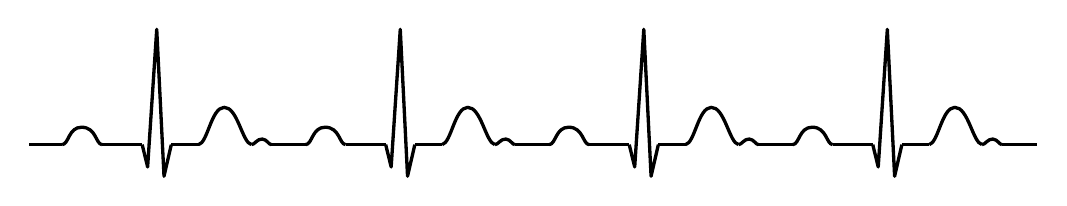
\begin{tikzpicture}[line join=round, x=2pt, y=-2pt]
    \tikzset{
        normal ecg/.pic={
            \draw (0,455.0021) -- (11.8345,455.0021);
            \draw (11.8345,455.0021) .. controls (14.2834,454.8958) and
              (14.1385,448.7114) .. (18.8842,448.7114) .. controls (24.2116,448.7114) and
              (23.9695,454.8958) .. (26.3035,455.0021);
            \draw (26.3035,455.0021) -- (40.7723,455.0021);
            \draw (40.7723,455.0021) -- (42.7455,463.0645) -- (46.0339,413.3461)
              -- (48.6647,466.4235) -- (51.2955,455.0021);
            \draw (51.2955,455.0021) -- (61.1605,455.0021);
            \draw (61.1605,455.0021) .. controls (64.4487,454.3298) and
              (65.7118,441.6860) .. (70.3679,441.5241) .. controls (75.2428,441.3542) and
              (76.9447,454.3301) .. (80.2329,455.0021);
            \draw  (80.2329,455.0021) .. controls (81.4852,455.0021) and
              (82.2677,452.8462) .. (84.1792,452.9863) .. controls (85.8717,453.1101) and
              (86.4830,455.0021) .. (87.4678,455.0021);
            \draw (87.4678,455.0021) -- (100,455.0021);
        }
    }
    \foreach \x in {0,...,3}{
    \pic [very thick, scale=0.5] at (\x*44, 0) {normal ecg};
    }
    \end{tikzpicture}

\end{document}
